\chapter{Final model}
	\section{Blending the IDM and MOBIL}
		Until this point all simulations were run in a one lane imaginary road. However to be able to represent real traffic situations multi lane roads has to be considered as mentioned in the introduction. In a road with multiple lanes IDM can describe the longitudinal and MOBIL the transversal motions. For a starting point let us revisit the model used previously:
		\begin{equation}
			\dot{y}=
			\begin{pmatrix}
			v_0\\
			0\\
			f_1(v_{2})\\
			f_2(x_{2}, v_{2},x_{1}, v_{1})\\
			f_1(v_{3})\\
			f_2(x_{3}, v_{3},x_{2}, v_{2})\\
			\vdots\\
			f_1(v_{\rm n-1})\\
			f_2(x_{n-1}, v_{n-1},x_{n-2}, v_{n-2})\\
			f_1(v_{\rm n})\\
			f_2(x_{n}, v_{n},x_{n-1}, v_{n-1})
			\end{pmatrix}\,.
			\label{eq:n_ode_math_revisit}
		\end{equation}
		As Equation \ref{eq:n_ode_math_revisit} shows there is a criterion on the car indexing.  Namely n-1-th vehicle is always the leader of n-th car. Every car is stored in an array called \textit{definition array} with their identifiers,  current and target lanes, initial positions and velocities, and parameters. An example of this definition array can be seen in Table \ref{tab:definition_array}.
		\begin{table}
			\begin{center}
				\begin{tabular}{ |c|c|c|c|c|c| }
					\hline
					Id & Current lane & Target lane & Initial position & Initial velocity& IDM params\\
					$[-]$ & $[-]$ & $[-]$ & $[m]$ & $[m/s]$ & $[-]$\\
					\hline
					1 & 1 & 0 & 100 & 0 & ...\\
					2 & 2 & 0 & 50 & 0 & ...\\
					\vdots & \vdots & \vdots & \vdots & \vdots & \vdots\\
					n - 1 & 1 & 0 & 200 & 0 & ...\\
					n & 1 & 0 & 0 &  & ...\\
					\hline
				\end{tabular}
			\end{center}
			\caption{Definition array example}
			\label{tab:definition_array}
		\end{table}
		Since there were no lane changes until this point, the indexing condition held. However this criterion cannot be satisfied where changing lanes are allowed. Instead of this condition a new function is introduced. The suggested method is capable of calculating which car is the leader of an other vehicle. So from now on the simulator relies on this function instead of the order of car models in the definition array.
		\subsection*{Determining the leader vehicle}
		The previously mentioned function does the following steps
		\begin{itemize}
			\item assembles and sorts a car model array with the required data by current vehicle position,
			\item searches for cars in the same lane,
			\item finds the row of the car by id,
			\item returns the row above (index - 1) if exists or nothing if there is no row above.
		\end{itemize}
		Let us call this function $g$. This $g$ function has one parameter, the id of the car whose leader vehicle is searched for. If there is leader than it returns exactly the same values as the IDM expects as parameters, namely the leading car's position and velocity.
		So Equation \ref{eq:n_ode_math_revisit} modifies as follows:
		\begin{equation}
			\dot{y}=
			\begin{pmatrix}
			f_1(v_1)\\
			f_2(x_{1}, v_{1},g(\id_1))\\
			f_1(v_2)\\
			f_2(x_{2}, v_{2},g(\id_2))\\
			f_1(v_2))\\
			f_2(x_{3}, v_{3},g(\id_3))\\
			\vdots\\
			f_1(v_{n-1}))\\
			f_2(x_{n-1}, v_{n-1},g(\id_{n-1}))\\
			f_1(v_n))\\
			f_2(x_{n}, v_{n},g(\id_{n}))
			\end{pmatrix}\,.
			\label{eq:n_ode_math_with_find_leading}
		\end{equation}
		As mentioned previously $g$ function can only return the expected parameters by $f$ if there is a leader car. This makes sense since someone has to be the very first in every single time step. Consequently that cars longitudinal model has to be changed to handle that there is no car in front of it. It is handled by leaving the follower behavior out of the equation \ref{eq:aidm}. So it will not need the leader vehicle's parameters. This means that the leader cars in their lanes will always be in free acceleration state. That is coinciding with reality. 
		\subsection*{Implementation of lane changing}
		The original n-car solver only calculated and stored the \textbf{y} vector which contained the position and velocity values at each time step. Since lane changes came into picture that wont be enough. Consequently, two more vectors needs to be stored. One for the current lane (named $\vcl$) and one for the target lane (named $\vtl$) which can keep track of the lane changes. $\vcl$ will store the lane numbers of the vehicle's current lane. $\vtl$ will contain the target lane identifier when a car is changing lane, otherwise it will have zero value. Figures \ref{fig:stage1ofchanginglanes}, \ref{fig:stage2ofchanginglanes}, \ref{fig:stage3ofchanginglanes} show the stages of a lane change example.
		\begin{figure}[ht]
			\begin{center}
				\begin{minipage}{.65\textwidth}
					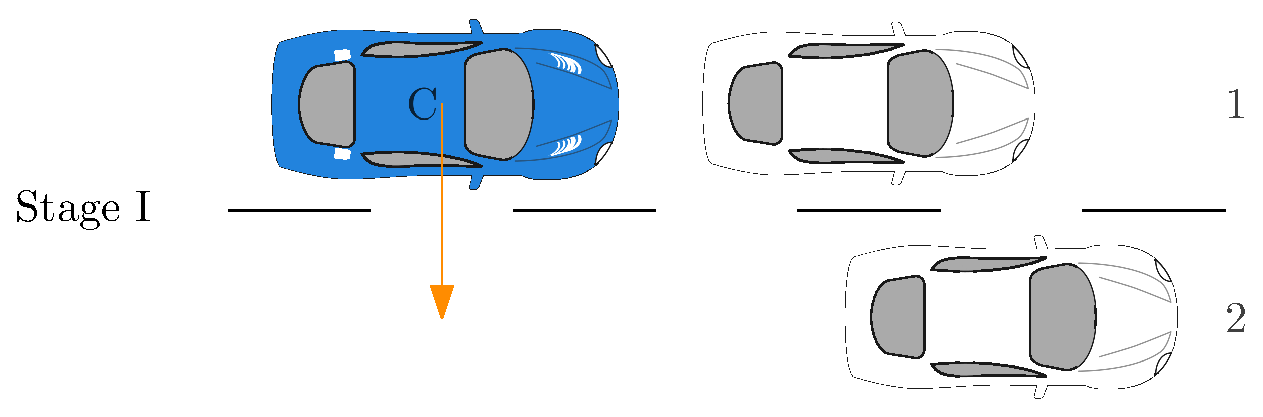
\includegraphics[width=\textwidth]{common/stages_of_lane_changes_1}
				\end{minipage}\quad
				\begin{minipage}{.3\textwidth}
					\begin{tabular}{ |c|c|c|c| }
						\hline
						Id &  $\vcl$ & $\vtl$ & ... \\
						$[-]$ & $[-]$ & $[-]$ & ...\\
						\hline
						$\vdots$ & $\vdots$ & $\vdots$ & \vdots\\
						$C$ & $2$ & $0$ & ...\\
						$\vdots$ & $\vdots$ & $\vdots$ & \vdots\\
						\hline
					\end{tabular}
				\end{minipage}
			\end{center}
			\caption{Stage I of changing lanes. Vehicle C is considering a lane change.}
			\label{fig:stage1ofchanginglanes}
		\end{figure}
		\begin{figure}[ht]
			\begin{center}
				\begin{minipage}{.65\textwidth}
					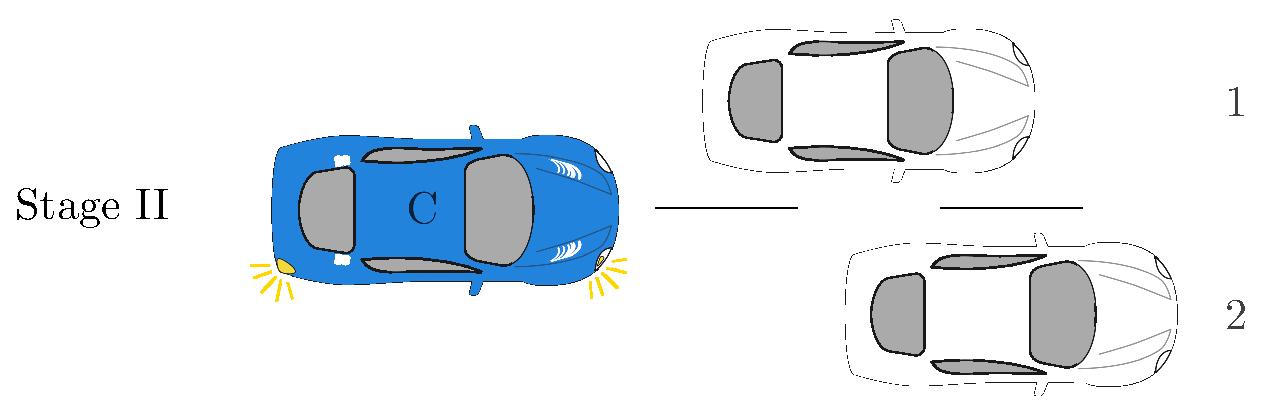
\includegraphics[width=\textwidth]{common/stages_of_lane_changes_2}
				\end{minipage}\quad
				\begin{minipage}{.3\textwidth}
					\begin{tabular}{ |c|c|c|c| }
						\hline
						Id &  $\vcl$ & $\vtl$ & ... \\
						$[-]$ & $[-]$ & $[-]$ & ...\\
						\hline
						$\vdots$ & $\vdots$ & $\vdots$ & \vdots\\
						$C$ & $2$ & $1$ & ...\\
						$\vdots$ & $\vdots$ & $\vdots$ & \vdots\\
						\hline
					\end{tabular}
				\end{minipage}
			\end{center}
			\caption{Stage II of changing lanes. Vehicle C changing lanes from lane 2 to lane 1. The row of vehicle C contains 2 in the current lane vector and 1 in the target lane vector.}
			\label{fig:stage2ofchanginglanes}
		\end{figure}
		\begin{figure}[ht]
			\begin{center}
				\begin{minipage}{.65\textwidth}
					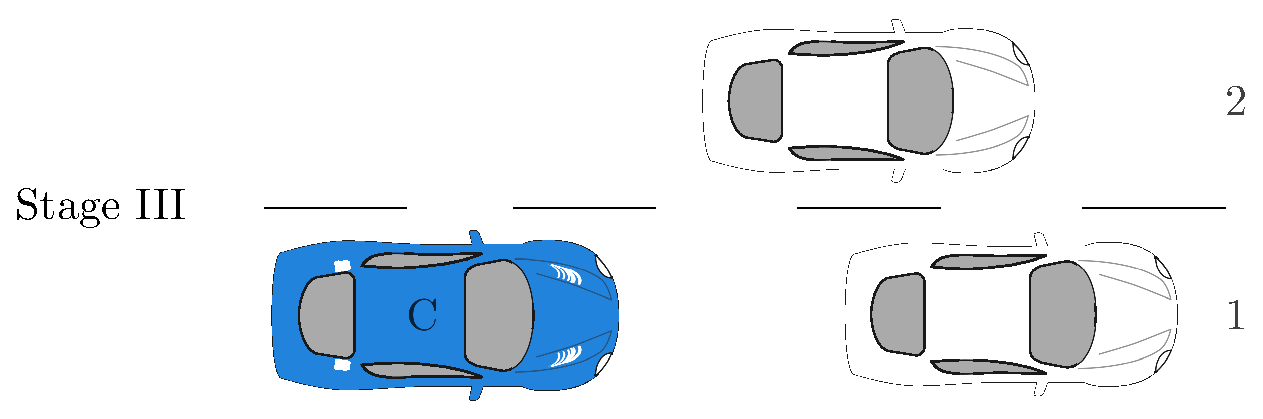
\includegraphics[width=\textwidth]{common/stages_of_lane_changes_3}
				\end{minipage}\quad
				\begin{minipage}{.3\textwidth}
					\begin{tabular}{ |c|c|c|c| }
						\hline
						Id &  $\vcl$ & $\vtl$ & ... \\
						$[-]$ & $[-]$ & $[-]$ & ...\\
						\hline
						$\vdots$ & $\vdots$ & $\vdots$ & \vdots\\
						$C$ & $1$ & $0$ & ...\\
						$\vdots$ & $\vdots$ & $\vdots$ & \vdots\\
						\hline
					\end{tabular}
				\end{minipage}
			\end{center}
			\caption{Stage III of changing lanes. Vehicle C has performed its lane change so the current lane vector will hold a value of 1 at the row of vehicle C, corresponding row of target lane vector will reset to zero.}
			\label{fig:stage3ofchanginglanes}
		\end{figure}
		\subsection*{Decision making}
		The updated model with vectors $\vcl$ and $\vtl$ is able to keep track of a multi lane traffic with lane changes. However the algorithm to fill those vectors correctly is not discussed yet. A lane change has multiple aspects like when does the driver wants to change or is it possible change lanes safely. Fortunately these two questions can be answered by simply implementing the algorithm of MOBIL.

		From the implementation point of view in every time step MOBIL calculates that a driver should change lanes or not. If a driver should change lanes based on the local traffic situation than the lane change starts by filling the corresponding row in the vector $\vtl$. For now the duration is neglected (more on that later). So the lane change will end in the next time step which means that the car's current lane value will be the target lane value and target lane resets to zero. It is worth mentioning that a lane changing car occupies both its current and target lane. So it will be the leader car in both current and target lane's immediate following cars.
	\section{Simulation of a traffic light situation}
		The model described in the previous section has been implemented in \textsc{Matlab}. The task is to test the solver through an interesting case like a red traffic light with 10 vehicles.
		\subsection*{Initial conditions}
		The initial conditions can be found in Table \ref{tab:case_1_definition_array}. The traffic situation can be seen on Figure \ref{fig:red_light_situation}. The front of the first car of each lane has been placed at zero position. Then every vehicle has been behind its leader by its traffic jam distance. The initial velocity of all cars is zero.  The IDM parameters of the simulated cars have been varied between realistic values. Also for the first time a bus has been introduced to traffic. From the model point of view a bus is only different from a regular car by its length and some of its IDM parameters like the maximum acceleration or duration of a lane change.
		
		Until now the simulator was running until a specific time point. It would be nice to run until when all of the cars have reached a specific distance. For example a traffic light situation is interesting for the first 100 meters. This has been implemented into the simulator as well.
		\begin{table}
			\begin{center}
				\begin{tabular}{ |c|c|c|c|c|c| }
					\hline
					Id & Current lane & Target lane & Initial position & Initial velocity& IDM params\\
					$[-]$ & $[-]$ & $[-]$ & $[m]$ & $[m/s]$ & $[-]$\\
					\hline
					1 & 1 & 0 & 0 & 0 & ..., L = 4.2, ... \\
					2 & 2 & 0 & 0 & 0 & ..., L = 4.4, ... \\
					3 & 1 & 0 & -5.4 & 0 & ..., L = 20, ... \\
					4 & 2 & 0 & -5.5 & 0 & ..., L = 4.1, ... \\
					5 & 1 & 0 & -26.4 & 0 & ..., L = 4.3, ... \\
					6 & 2 & 0 & -10.9 & 0 & ..., L = 4.5, ... \\
					7 & 1 & 0 & -31.9 & 0 & ..., L = 4.6, ... \\
					8 & 2 & 0 & -16.5 & 0 & ..., L = 4.2, ... \\
					9 & 1 & 0 & -37.7 & 0 & ..., L = 4.3, ... \\
					10 & 2 & 0 & -21.7 & 0 & ..., L = 4.4, ... \\
					\hline
				\end{tabular}
			\end{center}
			\caption{Initial conditions of Case 1}
			\label{tab:case_1_definition_array}
		\end{table}
		\begin{figure}
			\centering
			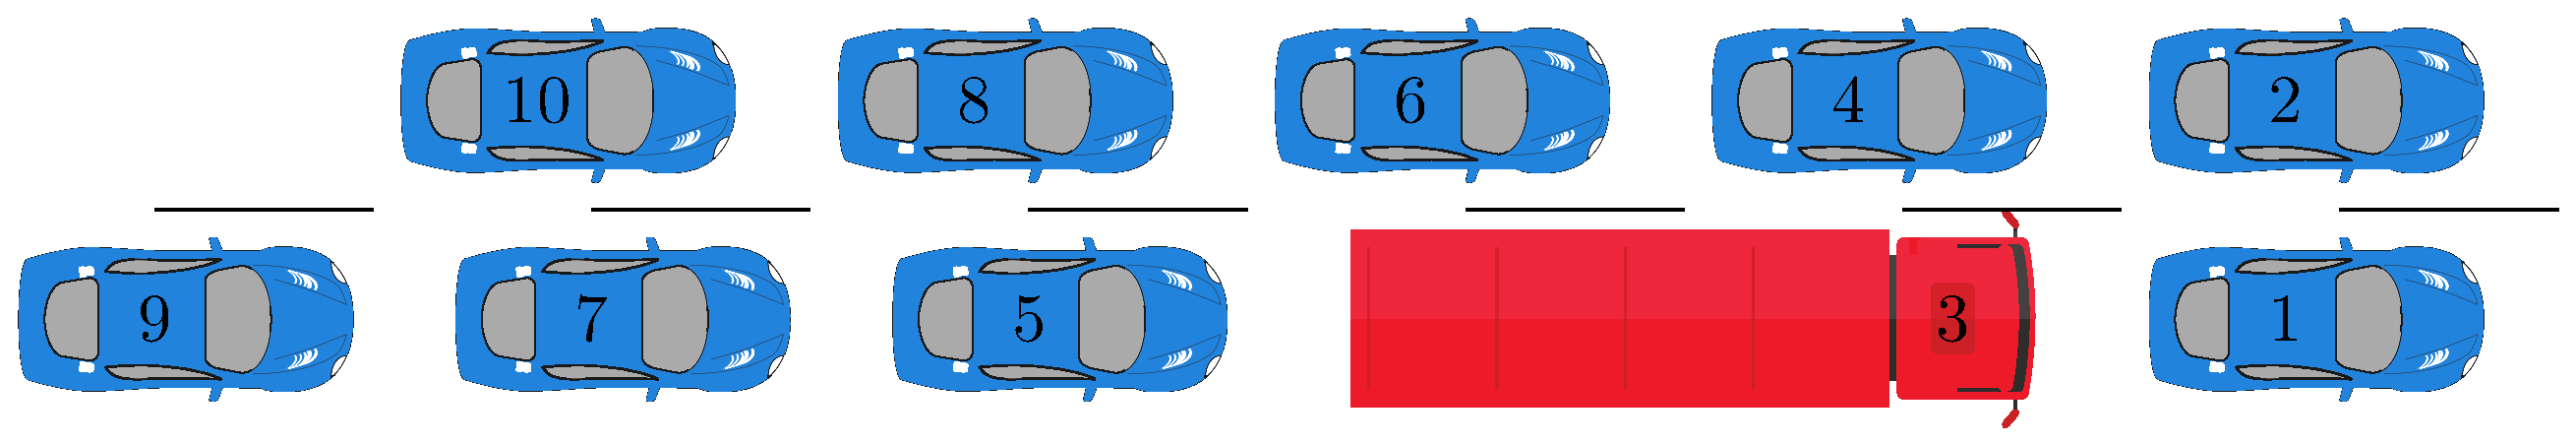
\includegraphics[width=\textwidth]{common/traffic_light_case_1}
			\caption{Red light situation with 10 vehicles}
			\label{fig:red_light_situation}
		\end{figure}
		\begin{figure}
			\centering
			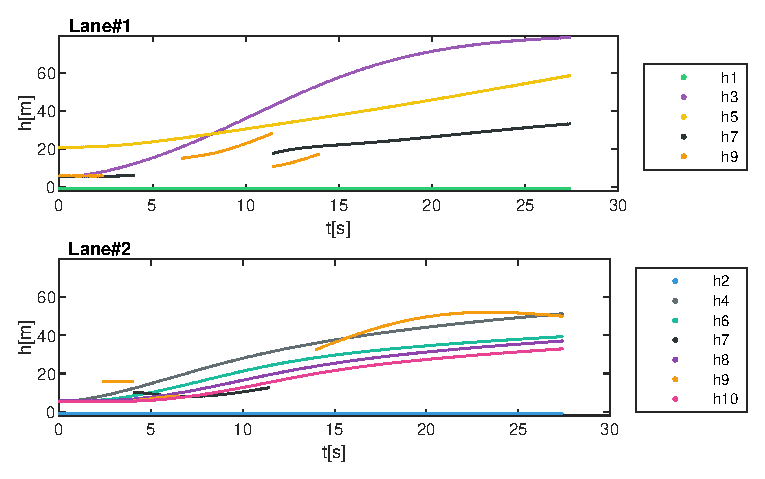
\includegraphics[width=0.8\textwidth]{eemobil/simh_case1}
			\caption{Red light traffic. Headway of the vehicles respect to their position in lanes}
			\label{fig:red_light_situationh}
		\end{figure}
		\begin{figure}
			\centering
			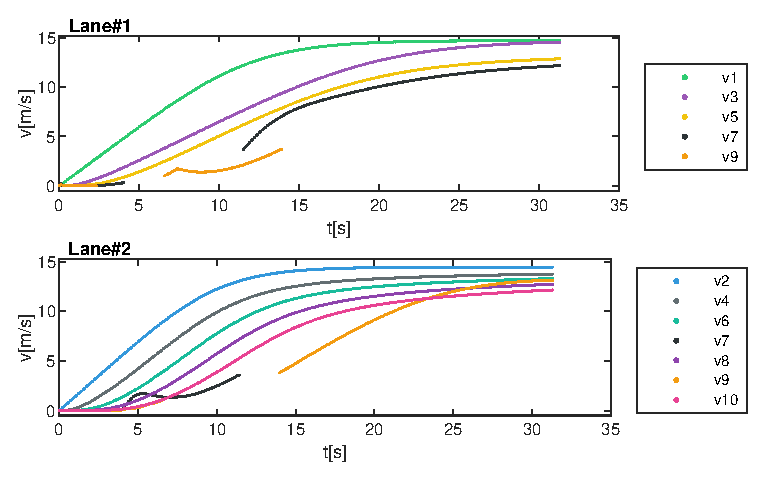
\includegraphics[width=0.8\textwidth]{eemobil/simv_case1}
			\caption{Red light traffic. Velocity of the vehicles respect to their position in lanes}
			\label{fig:red_light_situationv}
		\end{figure}
		\begin{figure}
			\centering
			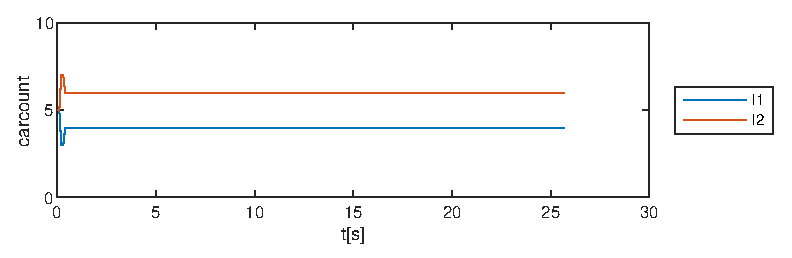
\includegraphics[width=0.8\textwidth]{eemobil/simcc_case1}
			\caption{Red light traffic. Number of cars in lanes }
			\label{fig:red_light_situationcc}
		\end{figure}
		\subsection*{Summary of the result}
		The traffic situation was successfully simulated. However post processing of the result turned out to be kind of a challenging task. The usage of the previous figures is not illustrating enough the traffic. To make it easy to understand the motions of the vehicles, the headway and velocity figures have been divided into two parts. One figure shows the headway of the cars in one lane the other figure shows the other lane. When a vehicle changes lanes its curve breaks and disappears from one figure and continues on the other. The headway and velocity diagrams can be seen on Figure \ref{fig:red_light_situationh} and \ref{fig:red_light_situationv}. Notice that the first cars of each lanes have zero headway since there is no vehicle in front of them.  Another figure was made to emphasize the lane changes during the simulation. Figure \ref{fig:red_light_situationcc} shows the number of vehicles in each lane. Notice that one function is opposite of the other.
		\section{Effect of the time step size on solutions}
		A numerical solution should be independent from the time step. Thus a time step independence analysis has been carried out. What practically it means is that one particular simulation should be run multiple times with decreasing step size. If the solution is converged than it can be said that the model is step size independent. The default value of the step size was 0.1 second. The simulations were run with the values defined in Table \ref{tab:timestepsizes}.
		Using the same parameters and initial conditions as before, the analysis has been performed. The result can be seen on Figure \ref{fig:tsip}, \ref{fig:tsiv}, \ref{fig:tsipr}, \ref{fig:tsivr} and \ref{fig:tsit}.
		\begin{table}[ht]
			\begin{center}
				\begin{tabular}{ |c||c|c|c|c|c|c|}
					\hline
					&1. & 2. & 3. & 4. & 5. & 6.\\
					\hline
					dt[s]& $0.4$ & $0.2$ & $0.1$ & $0.05$ & $0.025$ & $0.0125$\\
					\hline
				\end{tabular}
			\end{center}
			\caption{Step sizes}
			\label{tab:timestepsizes}
		\end{table}
		\begin{figure}[ht]
			\centering
			\begin{minipage}{.5\textwidth}
				\centering
				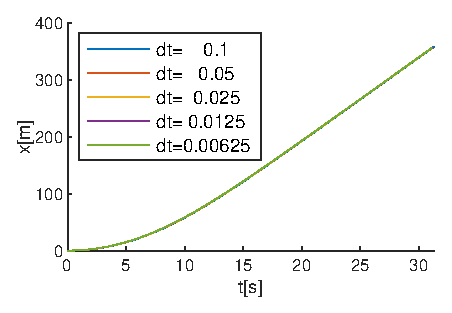
\includegraphics{eemobil/timestepi_p}
				\caption{Position of car 5}
				\label{fig:tsip}
			\end{minipage}\hfill
			\begin{minipage}{.5\textwidth}
				\centering
				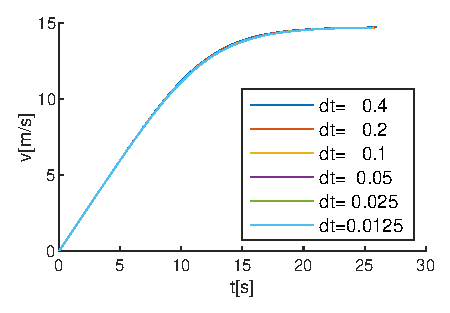
\includegraphics{eemobil/timestepi_v}
				\caption{Velocity of car 5}
				\label{fig:tsiv}
			\end{minipage}
		\end{figure}
		\begin{figure}
			\centering
			\begin{minipage}{.5\textwidth}
				\centering
				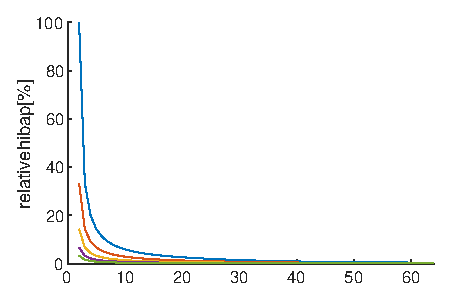
\includegraphics{eemobil/timestepi_relative_p}
				\caption{Relative error of position}
				\label{fig:tsipr}
			\end{minipage}\hfill
			\begin{minipage}{.5\textwidth}
				\centering
				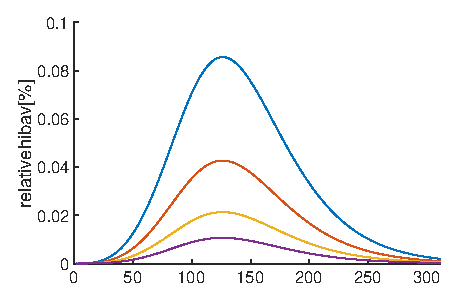
\includegraphics{eemobil/timestepi_relative_v}
				\caption{Relative error of velocity}
				\label{fig:tsivr}
			\end{minipage}
		\end{figure}
		\begin{figure}
			\centering
			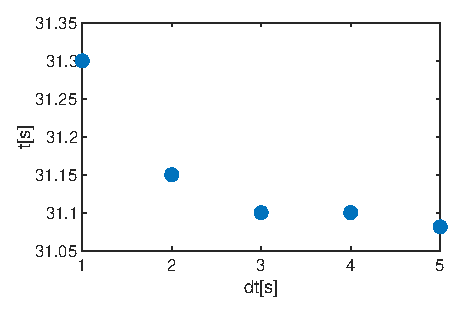
\includegraphics{eemobil/timestepi_t}
			\caption{Time step independence. Elapsed time for 100 meters}
			\label{fig:tsit}
		\end{figure}
		\section{Simulator improvements}
		The simulator works as expected. It is capable of simulating a multi lane traffic with lane changes. But there are some human driver behaviors that can be modeled slightly better, thus making the simulator  more realistic.
		\subsection{Improvement I}
		As mentioned previously the duration of a lane change is not modeled or implemented yet.  However it must be implemented since it has probably a great impact on the overall traffic outcome. It makes the simulator a bit more reasonable too. The actual duration of the lane change should be defined as a driver specific parameter in seconds. A typical value is 2 to 4 sec. After a lane change has started (by filling the corresponding row of the target lane vector) the simulator is checking the elapsed time in every time step for the lane changing vehicle. The simulator will end the lane change when the elapsed time has exceeded the lane change duration. To see the effect of this improvement the same configuration was simulated with the same initial conditions as before, only the newly introduced lane change duration parameters were added. See Table \ref{tab:lane_change_duration}.
		\begin{table}
			\begin{center}
				\begin{tabular}{ |c|c|c| }
					\hline
					Id & ... & Lane change duration\\
					$[-]$ & & [s]\\
					\hline
					1 & ... & 2.0\\
					2 & ... & 2.5\\
					3 & ... & 4.0\\
					4 & ... & 3.4\\
					5 & ... & 2.9\\
					6 & ... & 3.3\\
					7 & ... & 4.0\\
					8 & ... & 3.2\\
					9 & ... & 2.3\\
					1 & ... & 3.9\\
					\hline
				\end{tabular}
			\end{center}
			\caption{Initial conditions of Case 2}
			\label{tab:lane_change_duration}
		\end{table}
		
		Results of the simulation can be seen on Figure \ref{fig:red_light_situationh_impr1}, \ref{fig:red_light_situationv_impr1} and \ref{fig:red_light_situationcc_impr1}.
		\begin{figure}
			\centering
			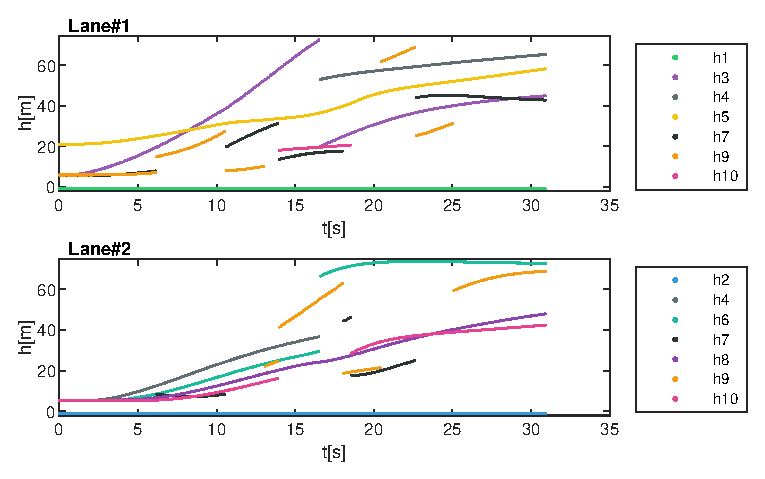
\includegraphics[width=0.8\textwidth]{eemobil/simh_case2}
			\caption{Red light traffic. Headway of the vehicles respect to their position in lanes}
			\label{fig:red_light_situationh_impr1}
		\end{figure}
		\begin{figure}
			\centering
			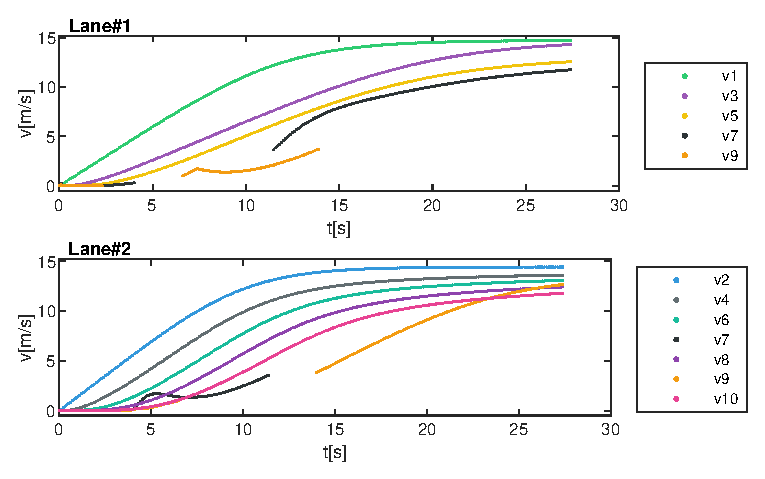
\includegraphics[width=0.8\textwidth]{eemobil/simv_case2}
			\caption{Red light traffic. Velocity of the vehicles respect to their position in lanes}
			\label{fig:red_light_situationv_impr1}
		\end{figure}
		\begin{figure}
			\centering
			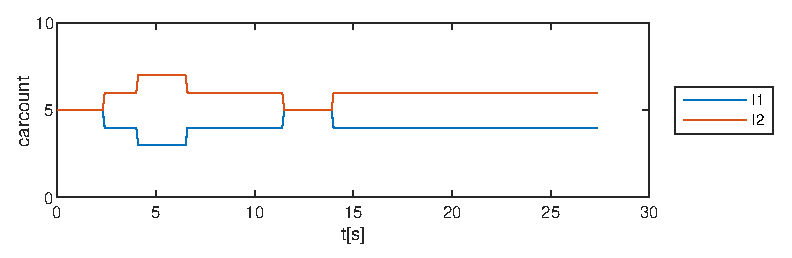
\includegraphics[width=0.8\textwidth]{eemobil/simcc_case2}
			\caption{Red light traffic. Number of cars in lanes }
			\label{fig:red_light_situationcc_impr1}
		\end{figure}
		\subsection{Improvement II ?!!!!!!}
		Currently the acceleration value of a vehicle during a lane change is calculated by its leader only. However in a real situation a driver changes lane because he would like to accelerate. So instead of calculating the acceleration based on the current leader only, both the current and the future leader accelerations should take into account. A reasonable approximation could be that the car's current acceleration is a weighted average by the elapsed time from the duration of the lane change between the acceleration value of the current and  future leader. A mathematical expression of this improvement would look like:
		\begin{equation}
			a=a_{\rm c} \cdot \left(1-\frac{t_{\rm e}}{t_{\rm d}}\right) + a_{\rm f}\cdot \frac{t_{\rm e}}{t_{\rm d}}\,,
			\label{eq:weighted_average}
		\end{equation}
		where $a_{\rm c}$ is the acceleration considering only the current leader vehicle, $a_{\rm f}$  is the acceleration considering only the future leader vehicle. $t_e$ and $t_d$ is the elapsed and total time of the lane change. Based on Equation \ref{eq:weighted_average} the improvement has been implemented in the simulator. This feature has been added with a toggle if one wishes to turn off in the future.
		\subsection{Improvement III}
		The other area which can be developed is related to the attention of the drivers to the road. The model currently assumes that everyone is paying attention to the driving always. This is not the case in real life at all. There are several factors which can distract the driver's attention. Some of these activities could be eating, interacting with radio or gps, looking at a roadside object or messaging on the phone. These activities most likely to have an effect on the road so it is worth to implement. The model will assume that if a driver is distracted with something then it cannot take any attention to its longitudinal nor the transversal motions. So the car will go ahead with the same speed and zero acceleration when it is nobody ahead and even if its leader is braking.The actual implementation is quite simple. A new array is introduced which will contain the time intervals. These represent the the time when a driver is not paying attention to driving. Whenever a driver is not paying attention the simulator will keep its speed.

		 Another problem is that driving - as discussed earlier - consists of two parts, longitudinal and transversal motions. Probably drivers have to divide their attention and focus on only one at a time. It seems right to say that everyone is capable of paying attention to longitudinal and transversal motions at the same time when the speed is moderated. However when a driver is accelerating or decelerating above or below a certain point he will not care about changing lanes. This could be included in the lane changing algorithm. If Equation \ref{eq:attention_acceleration}  holds then the driver is capable of paying attention to lane changing otherwise he cannot.
		\begin{equation}
			|a|<a_{\rm tr}
			\label{eq:attention_acceleration}
		\end{equation}
		The current acceleration value is represented by $|a|$ and $a_{\rm p,tr}$ is threshold value which is typically between 0 and $\amax$ for a human driver.
	\section{Solution with improvements}
		\subsection*{Initial conditions}
		The initial conditions remained the same, except additional parameters were necessary to provide for the improvements. The initial conditions with the additional parameters can be found in Table \ref{tab:new_array}. The table contains the time intervals whenever a driver is not paying attention as well as the acceleration threshold value.
		\begin{table}
			\begin{center}
				\begin{tabular}{ |c|c|c|c| }
					\hline
					Id & ... & Driving without attention time intervals & $a_{\rm p,tr}$\\
					$[-]$ & & [s]& $\rm [m/s^2]$\\
					\hline
					1 & ... & 24-26 & 1.2 \\
					2 & ... & 0-2 & 1.2 \\
					3 & ... & 10-12 & 1.3 \\
					4 & ... & 0-3, 22-24, 25-25.5 & 1.3 \\
					5 & ... & 15-19 & 1.6 \\
					6 & ... & 15-16.5 & 1.6 \\
					7 & ... & 0-2 & 1.3 \\
					8 & ... & & 1.1 \\
					9 & ... & 0-3 & 1.3 \\
					1 & ... & 0-4,15-18.5 & 1.7 \\
					\hline
				\end{tabular}
			\end{center}
			\caption{Initial conditions of Case 2}
			\label{tab:new_array}
		\end{table}
		\begin{figure}
			\centering
			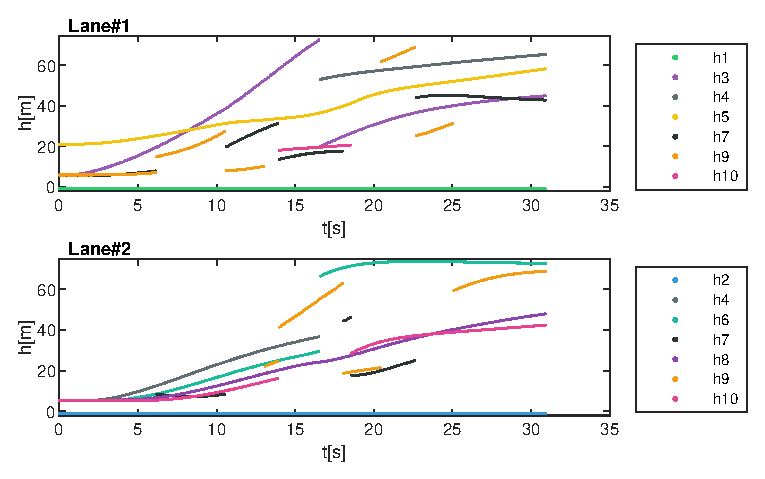
\includegraphics[width=0.8\textwidth]{eemobil/simh_case2}
			\caption{Red light traffic case 2. Headway of the vehicles respect to their position in lanes}
			\label{fig:red_light_situationh2}
		\end{figure}
		\begin{figure}
			\centering
			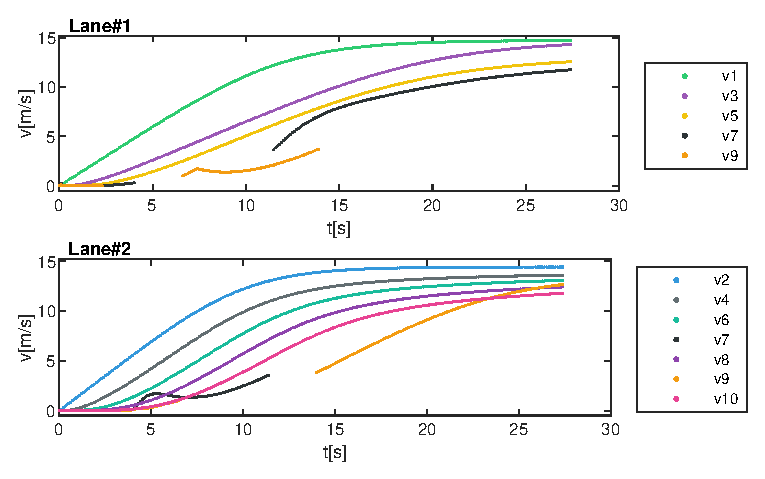
\includegraphics[width=0.8\textwidth]{eemobil/simv_case2}
			\caption{Red light traffic case 2. Velocity of the vehicles respect to their position in lanes}
			\label{fig:red_light_situationv2}
		\end{figure}
		\begin{figure}
			\centering
			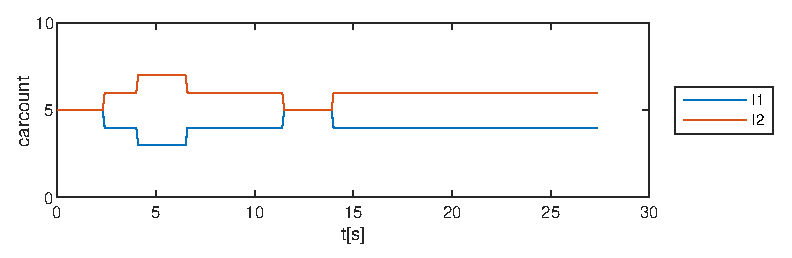
\includegraphics[width=0.8\textwidth]{eemobil/simcc_case2}
			\caption{Red light traffic case 2. Number of cars in lanes }
			\label{fig:red_light_situationcc2}
		\end{figure}
		\subsection*{Summary of the result}
		The results can be seen on Figure \ref{fig:red_light_situationh2}, \ref{fig:red_light_situationv2} and \ref{fig:red_light_situationcc2}.
		[TODO: Here comes the magnifier images.]
